\documentclass[conference]{IEEEtran}

\usepackage{amsmath,amssymb}
\usepackage{graphicx}
\usepackage{booktabs}
\usepackage{array}
\usepackage{cite}
\usepackage{url}

\newcommand{\TBD}{\textsc{TBD}}

\title{Anchor-Canvas Surface Fusion for Aperture-Limited Sand Reconstruction with a Frozen Geometry Foundation Model}

\author{
\IEEEauthorblockN{Author Name(s)}
\IEEEauthorblockA{Affiliation, City, Country\\
Email: author@example.com}
}

\begin{document}
\maketitle

\begin{abstract}
Low-texture surfaces observed through a rotating aperture expose a gap between feed-forward geometry prediction and usable surface reconstruction. A frozen geometry foundation model can predict depth and confidence, but direct multi-view fusion often turns small depth-scale differences and aperture occlusions into vertical ghosting, seam artifacts, and holes. This paper presents a training-free reconstruction layer that treats OmniVGGT as a frozen local geometry backend and places the technical contribution in the surrounding system modules. The proposed system has two coupled parts: a general stream wrapper with change masks, bucketed active windows, protected keyframes, and a hybrid hot/cold map; and an aperture-specific anchor-canvas pipeline that aligns images to a canonical 2-D coordinate system, corrects per-frame depth in overlap regions, and fuses a single height value per canonical cell. The method is designed for a practical sand-surface inspection sequence where cameras are uncalibrated, the observation aperture moves, and visible texture is partly photometric. On a retained 12-image case study, the static anchor-canvas path selects three keyframes, produces 440,911 points, removes unreliable boundary support, and reports zero detected internal holes. Overlap depth alignment reduces local median absolute residuals from 0.0278 and 0.0406 to 0.0030 and 0.0039 on two non-anchor frames. A streaming preview configuration processes subsequent frames in 0.973 s on average after backend loading, with an average changed-pixel ratio of 1.11\%. The paper also specifies a full 3-D reconstruction evaluation protocol, including accuracy, completeness, F-score, Chamfer distance, normal consistency, hole rate, seam discontinuity, runtime, and memory metrics, with placeholders for future ground-truth or reference-scan results.
\end{abstract}

\begin{IEEEkeywords}
3-D reconstruction, point cloud, streaming perception, depth fusion, homography alignment, low-texture surfaces, surface inspection
\end{IEEEkeywords}

\begin{figure*}[t]
\centering
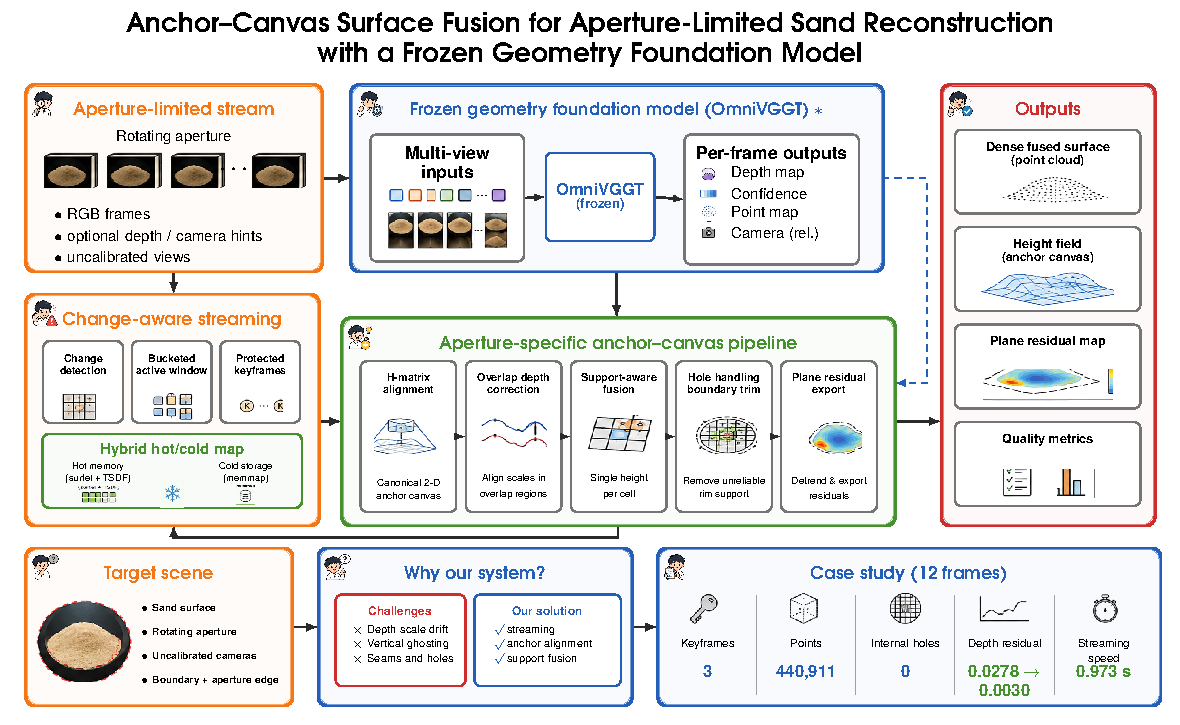
\includegraphics[width=\textwidth]{figures/reference_rebuild.pdf}
\caption{Main overview of the proposed reconstruction system. A frozen geometry backend provides local depth and confidence predictions, while the added modules perform stream selection, anchor-canvas alignment, overlap depth correction, support-aware fusion, boundary handling, and plane-residual export for aperture-limited sand reconstruction.}
\label{fig:main_overview}
\end{figure*}

\section{Introduction}
Feed-forward visual geometry models have changed the cost structure of 3-D reconstruction. Instead of running a full optimization pipeline every time a new set of images arrives, a model can predict cameras, depth maps, point maps, and confidence estimates from one or more images in a single forward pass \cite{wang2025vggt}. OmniVGGT extends this direction by accepting auxiliary depth and camera modalities through a GeoAdapter while keeping the base representation compatible with the original model family \cite{peng2025omnivggt}. These models are useful as local geometry predictors. They do not, by themselves, solve the system problem of maintaining a stable scene representation under constrained capture.

The target scene in this project is deliberately difficult for raw multi-view fusion. The input is a short image sequence of sand captured through a rotating observation aperture. The camera intrinsics are not known, the aperture hides parts of the surface, and the true sand boundary is not the visible dark aperture boundary. The target surface is also low texture in a geometric sense. Image-level texture can be strong because sand has color, illumination, and material patterns, but those patterns do not necessarily correspond to measurable height relief. Directly fusing per-frame geometry therefore creates predictable failure modes: multiple vertical layers, frame-boundary seams, missing interior support, and apparent global bending.

The design problem reduces to two technical challenges. They are not model-training challenges, because the geometry predictor is kept frozen. They are system and fusion challenges: deciding which observations should be processed as the stream evolves, and making locally predicted depths compatible enough to form a stable surface representation.

First, a frozen model does not know which historical frames should be revisited for each new observation. Sending the full sequence into a model is expensive, while sending only the newest frame loses geometric context. Second, for the aperture-limited sand scene, model-predicted depth maps from different frames are not directly compatible. Even when image registration is good, depth scale and local residual differences can turn a near-planar surface into a thick point cloud.

The contribution of this paper is therefore outside the OmniVGGT model. The added modules are:
\begin{itemize}
\item A no-training streaming wrapper that converts a sequence of RGB frames, optional depth maps, and optional camera hints into local model calls and incremental map updates.
\item A change-aware active-window selector that keeps current frames, recent context, and protected anchors while avoiding full-history inference.
\item A hybrid block map that fuses changed, confidence-gated points into surfel and TSDF-like state, with hot memory and cold memmap storage.
\item A scene-specific anchor-canvas reconstruction path for aperture-limited sand inspection, including homography alignment, overlap depth correction, support-aware fusion, hole handling, boundary trimming, and plane-residual export.
\item A reproducible evaluation plan for current and future experiments, including 3-D reconstruction metrics whose results can be filled once ground truth or a scanned reference is available.
\end{itemize}

Figure~\ref{fig:main_overview} summarizes the full pipeline and marks the boundary between the frozen backend and the added reconstruction modules.

The paper does not claim a new foundation model. OmniVGGT remains a frozen backend. The research question is whether scene-aware modules around a frozen geometry model can improve reconstruction usability for a constrained inspection setting.

\section{Related Work}
\subsection{Feed-Forward Geometry Models}
VGGT demonstrated that a transformer can predict dense visual geometry attributes from one or more views, including camera parameters, depth, point maps, and point tracks \cite{wang2025vggt}. OmniVGGT adds auxiliary modalities such as camera and depth inputs through a GeoAdapter \cite{peng2025omnivggt}. Both works motivate using a learned geometry model as a local predictor. The present work takes a narrower systems view: the model is useful, but only as one component in a reconstruction pipeline that must handle temporal state, invalid boundaries, and scene-specific priors.

\subsection{Incremental Mapping}
Classical dense mapping systems separate local measurements from persistent map state. Voxblox incrementally integrates observations into signed distance fields for onboard planning \cite{oleynikova2017voxblox}. Open3D provides 3-D processing structures and implementations that are often used for practical point-cloud and volumetric pipelines \cite{zhou2018open3d}. The stream wrapper follows this principle. Model inference is local and episodic. Map state is long-lived, block-indexed, and updateable.

\subsection{Image Registration and Robust Fitting}
The aperture-specific path relies on image alignment before depth fusion. SIFT remains a standard feature descriptor for matching under scale and rotation changes \cite{lowe2004sift}. RANSAC is the standard robust model-fitting framework used to estimate transformations in the presence of outliers \cite{fischler1981ransac}. In this paper, homography estimation is not treated as full 3-D calibration. It defines a stable 2-D canonical canvas for a near-planar target.

\subsection{3-D Reconstruction Evaluation}
Large-scale reconstruction benchmarks evaluate accuracy, completeness, and precision-recall tradeoffs rather than only visual plausibility. Tanks and Temples popularized F-score style reporting for reconstructed geometry at specified distance thresholds \cite{knapitsch2017tanks}. ETH3D evaluates multi-view stereo using high-resolution imagery and reference scans \cite{schoeps2017eth3d}. This paper adopts the same general family of metrics for future experiments, but it reports current results honestly as a case study because the retained sand sequence has no metric ground truth.

\section{Problem Formulation}
\subsection{Input and Output}
Let the input sequence be
\begin{equation}
\mathcal{I}=\{I_t\}_{t=1}^{T},
\end{equation}
where $I_t \in \mathbb{R}^{H_t \times W_t \times 3}$ is an RGB image. Some frames may also include depth $D_t$, intrinsics $K_t$, and camera-to-world pose $E_t$, but the aperture-limited sand sequence used here does not assume reliable side inputs. The desired output is a colored point set
\begin{equation}
\mathcal{P}=\{(x_j,y_j,z_j,c_j)\}_{j=1}^{N}
\end{equation}
or, in the anchor-canvas case, a height field $Z(u)$ over canonical image coordinates $u=(u_x,u_y)$.

\subsection{Scene Assumptions}
The method uses three assumptions. The first is geometric: the inspected surface is near planar at the macro scale. Fine relief may exist, but the global surface should be thin. The second is observational: the rotating aperture changes visible support, so image boundaries cannot be interpreted as true object boundaries. The third is computational: the geometry model is frozen and expensive enough that repeated full-sequence inference should be avoided.

\subsection{Failure Modes}
The raw failure modes define the design targets:
\begin{itemize}
\item \textbf{Depth-scale mismatch.} Per-frame depth maps may have different offsets or scales, producing layered geometry after fusion.
\item \textbf{Pose or registration drift.} Model-predicted camera fusion can be unstable for low-texture near-planar surfaces.
\item \textbf{Aperture holes.} Occluder-induced missing regions can become internal holes if support is not regularized.
\item \textbf{False boundaries.} The dark aperture rim is not a sand boundary, so naive masks can remove valid surface or keep invalid edges.
\item \textbf{Photometric false relief.} Brightness and texture do not always imply height, so appearance-based detail must be kept separate from metric geometry.
\end{itemize}

\section{Streaming Reconstruction Framework}
\subsection{Data Model}
The general stream wrapper uses typed packets. Each packet contains a frame id, timestamp, RGB image, optional depth, optional intrinsics, optional pose, and metadata. A selected window is a bounded list of window frames with two index sets: frames that provide camera supervision and frames that provide depth supervision. This matches the frozen backend interface while keeping model calls small.

\subsection{Change Detection}
For frame $t$, the change detector compares the current RGB image against either the previous frame or a reprojected reference. It combines image residual, depth residual, optical flow magnitude, and confidence:
\begin{equation}
s_t(p)=\lambda_I r^I_t(p)+\lambda_D r^D_t(p)+
\lambda_F \frac{\|u_t(p)\|_2}{\tau_F}+\lambda_C(1-c_{t-1}(p)).
\label{eq:score}
\end{equation}
The binary mask is
\begin{equation}
\begin{aligned}
M_t(p)=\mathbf{1}\big[
&r^I_t(p)>\tau_I \vee r^D_t(p)>\tau_D\\
&\vee \|u_t(p)\|_2>\tau_F
\vee c_{t-1}(p)<\tau_C
\big].
\end{aligned}
\end{equation}
Morphological dilation expands the mask to include local support around changed pixels. The mask is also projected into coarse block hints:
\begin{equation}
\mathcal{B}_t=\left\{\left(\left\lfloor\frac{p_x}{b}\right\rfloor,
\left\lfloor\frac{p_y}{b}\right\rfloor,0\right):M_t(p)=1\right\}.
\end{equation}
where $b$ is the image-space block size.

\subsection{Active Window Selection}
The active-window selector bounds context length without discarding all history. It scores each candidate frame $f$ as
\begin{equation}
\begin{aligned}
q(f)=&\exp\left(-\frac{\Delta t_f}{\tau_r}\right)
+\beta_o r_o(f)
+\beta_c \mathbf{1}_{\mathrm{camera}}(f)\\
&+\beta_d \mathbf{1}_{\mathrm{depth}}(f)
+\beta_a \mathbf{1}_{\mathrm{anchor}}(f)
+\beta_m \bar{c}_f,\\
r_o(f)=&\frac{|\mathcal{B}_f \cap \mathcal{B}_t|}
{\max(|\mathcal{B}_t|,1)} .
\end{aligned}
\label{eq:window_score}
\end{equation}
The current frame is always included. At least one anchor frame is included if one exists. The window size is rounded to one of four buckets, 3, 4, 6, or 8 frames, which keeps tensor shapes predictable for backend warmup.

\begin{figure}[t]
\centering
\footnotesize
\begin{tabular}{p{0.94\linewidth}}
\toprule
\textbf{Algorithm 1: Change-aware streaming update}\\
\midrule
Input: packet $I_t$, frame history $\mathcal{H}$, keyframes $\mathcal{K}$, map $\mathcal{M}$.\\
1. Apply optional rotation and height preprocessors.\\
2. Resize image and optional depth to a bucketed shape.\\
3. Compute change mask $M_t$ with Eq.~\eqref{eq:score}.\\
4. Select a bucketed active window using Eq.~\eqref{eq:window_score}.\\
5. If the change ratio is below the no-change threshold, skip model inference.\\
6. Run the frozen OmniVGGT backend on the selected window.\\
7. Extract current-frame points, keep changed pixels, and gate by confidence.\\
8. Assign points to spatial blocks and fuse them into the hybrid map.\\
9. Promote keyframes and evict cold non-anchor blocks if needed.\\
Output: updated map and per-frame timing metrics.\\
\bottomrule
\end{tabular}
\caption{General streaming wrapper. The model is called only on a bounded active window; persistent state remains outside the model.}
\label{fig:alg_stream}
\end{figure}

\subsection{Hybrid Map Fusion}
Let $v$ be voxel size and $R$ the block resolution. A point $x \in \mathbb{R}^3$ maps to a block key
\begin{equation}
b(x)=\left\lfloor \frac{x}{vR}\right\rfloor.
\end{equation}
Only confidence-gated changed points are fused:
\begin{equation}
\mathcal{P}_t^{+}=\{x_p: M_t(p)=1, c_t(p)\ge \tau_c\}.
\end{equation}
For surfel-style fusion, an existing block point with weight $w$ and a new observation with weight $w_o$ are updated by
\begin{equation}
\begin{aligned}
x'&=\frac{wx+w_o x_o}{w+w_o},\\
c'&=\frac{wc+w_o c_o}{w+w_o},\\
w'&=\min(w+w_o,w_{\max}).
\end{aligned}
\end{equation}
The observation weight includes prediction confidence and an age penalty:
\begin{equation}
w_o=c_o \exp(-\lambda_{\mathrm{age}}\Delta t).
\end{equation}
Blocks marked as anchor blocks are protected from ordinary least-recently-used eviction. Inactive blocks may be written to a cold memmap store and restored later.

\section{Anchor-Canvas Method for Aperture-Limited Sand}
\subsection{Method Overview}
The anchor-canvas path is designed for sequences without reliable camera intrinsics or depth side inputs. It avoids using frozen-model camera estimates as global fusion coordinates. Instead, it uses image registration to define a canonical 2-D coordinate system, then treats model depth as a relative height signal that must be aligned before fusion.

\begin{figure}[t]
\centering
\footnotesize
\begin{tabular}{p{0.94\linewidth}}
\toprule
\textbf{Algorithm 2: Anchor-canvas static reconstruction}\\
\midrule
Input: image sequence $\{I_t\}$, anchor index $a$, maximum keyframes $K$.\\
1. Estimate pairwise homographies with feature matching and RANSAC.\\
2. Score candidate keyframe sets by coverage, compactness, hole penalty, and graph distance.\\
3. Choose an anchor image and selected keyframes.\\
4. Warp each selected frame into the anchor canvas.\\
5. Run the frozen backend on selected frames to obtain depth and confidence.\\
6. Align each non-anchor depth map to the anchor over overlap cells.\\
7. Fuse depth with confidence, feathering, and consistency weights.\\
8. Enforce support constraints, fill internal holes, and trim unreliable boundaries.\\
9. Fit a robust plane and export residual height as a colored point cloud.\\
Output: point cloud, alignment report, keyframe report, and diagnostics.\\
\bottomrule
\end{tabular}
\caption{Static anchor-canvas reconstruction. This path favors quality and diagnostics over low latency.}
\label{fig:alg_anchor}
\end{figure}

\subsection{Pairwise Alignment Graph}
For each image pair $(i,j)$, the implementation estimates a homography $H_{i \rightarrow j}$ using matched local features and robust inlier selection. An edge is accepted when it satisfies minimum inlier count, maximum median reprojection error, and minimum overlap constraints:
\begin{equation}
e_{ij}=1\quad \mathrm{if}\quad n_{ij}\ge n_{\min},\; \epsilon_{ij}\le \epsilon_{\max},\; o_{ij}\ge o_{\min}.
\end{equation}
The edge score is
\begin{equation}
\phi_{ij}=\frac{n_{ij}o_{ij}}{\epsilon_{ij}+\epsilon_0},
\end{equation}
where $\epsilon_0$ prevents division by zero. The selected anchor should be well connected in this graph.

\subsection{Keyframe Set Objective}
Candidate keyframe sets are scored by coverage, compactness, hole penalties, and distance from the anchor:
\begin{equation}
\begin{aligned}
J(\mathcal{K})=&\alpha_A A(\mathcal{K})
-\alpha_C C(\mathcal{K})
-\alpha_H H_{\mathrm{holes}}(\mathcal{K})\\
&-\alpha_N N_{\mathrm{holes}}(\mathcal{K})
-\alpha_G \sum_{k\in \mathcal{K}} d_G(k,a).
\end{aligned}
\label{eq:keyframe_objective}
\end{equation}
Here $A$ is union support area, $C$ penalizes an unnecessarily large or fragmented canvas, $H_{\mathrm{holes}}$ is total internal-hole area, $N_{\mathrm{holes}}$ is hole count, and $d_G$ is graph distance from anchor $a$. The retained output selects three frames because the third frame improves support while keeping overlap usable.

\subsection{Canonical Canvas}
The anchor image defines coordinates $u=(u_x,u_y)$. Each selected frame $i$ is warped to the anchor by
\begin{equation}
\bar{u} \sim H_{i\rightarrow a}\bar{p},
\end{equation}
where $\bar{p}$ and $\bar{u}$ are homogeneous image coordinates. This choice deliberately avoids a calibrated 3-D camera model. It is appropriate because the target is near planar and the desired output is a relative-scale surface.

\subsection{Overlap Depth Alignment}
Depth predicted by a frozen model is not directly comparable across uncalibrated views. For a non-anchor frame $i$, let $\Omega_i$ be overlap cells where both anchor depth and warped frame depth are valid. A frame-level alignment solves
\begin{equation}
(\alpha_i,\beta_i)=\arg\min_{\alpha,\beta}
\sum_{u\in \Omega_i}\rho(\alpha z_i(u)+\beta-z_a(u)),
\label{eq:affine_depth}
\end{equation}
where $\rho$ is a robust penalty. The implementation also permits a low-order local residual correction:
\begin{equation}
\tilde{z}_i(u)=\alpha_i z_i(u)+\beta_i+\eta_i(u).
\end{equation}
The local correction is estimated only from overlap support and is bounded to avoid bending the anchor surface. By default, the anchor depth is locked. This prevents secondary frames from reshaping the reference surface.

\subsection{Support-Aware Soft Fusion}
Each valid warped observation contributes a weight
\begin{equation}
w_i(u)=
c_i(u)^{\gamma_c}\,
f_i(u)^{\gamma_f}\,
\exp\left(-\frac{| \tilde{z}_i(u)-\hat{z}(u)|}{\sigma_z}\right),
\label{eq:fusion_weight}
\end{equation}
where $c_i$ is model confidence, $f_i$ is a feathered distance-to-boundary term, and $\hat{z}$ is the current consensus estimate. The fused height is
\begin{equation}
Z(u)=\frac{\sum_i w_i(u)\tilde{z}_i(u)}{\sum_i w_i(u)+\epsilon}.
\end{equation}
The support count is
\begin{equation}
S(u)=\sum_i \mathbf{1}[w_i(u)>0].
\end{equation}
The recommended static configuration requires $S(u)\ge 2$ for retained interior support. Narrow support gaps are closed, internal holes under a maximum area are filled, and an outer boundary band is trimmed.

\subsection{Plane-Residual Export}
The output should be a thin relative surface, not a globally bent depth sheet. A plane
\begin{equation}
\pi(x,y)=\theta_1 x+\theta_2 y+\theta_3
\end{equation}
is fitted with robust inlier selection:
\begin{equation}
\theta^*=\arg\min_{\theta}\sum_{u\in \Omega} \rho(Z(u)-\pi(x(u),y(u))).
\end{equation}
Residual height is
\begin{equation}
r(u)=Z(u)-\pi_{\theta^*}(x(u),y(u)).
\end{equation}
Residuals are clipped at a multiple of the median absolute deviation (MAD):
\begin{equation}
\hat{r}(u)=\mathrm{clip}(r(u), m-\kappa\,\mathrm{MAD},m+\kappa\,\mathrm{MAD}),
\end{equation}
where $m$ is the residual median. Clipping keeps XY support instead of deleting points, which avoids creating artificial holes.

\subsection{Optional Residual-Flow Detail}
The optional detail branch estimates local residual flow after homography alignment. If $\delta u_i(u)$ is the residual optical flow between anchor and frame $i$, a normalized scalar detail field is
\begin{equation}
d(u)=\mathrm{norm}\left(\sum_i \omega_i(u)\,g(\delta u_i(u))\right),
\end{equation}
and the displayed height becomes
\begin{equation}
r_{\mathrm{detail}}(u)=\hat{r}(u)+\lambda_d d(u).
\end{equation}
This branch is marked as visualization or relative micro-relief. It is not a calibrated physical-height estimate.

\section{Implementation Details}
\subsection{Backend Adapter}
The backend adapter attempts to load the local OmniVGGT model and checkpoint. If model import, checkpoint loading, CUDA initialization, or unsupported engine mode fails, it falls back to a deterministic mock backend. This makes tests and synthetic benchmarks independent of heavy model weights. For real runs, the adapter uses \texttt{torch.inference\_mode()} and CUDA autocast when BF16 or FP16 is selected.

\subsection{Shape Buckets}
The general stream wrapper uses target width, target size, and patch-multiple constraints to keep input tensors in a small set of shapes. This matters because frozen-model inference dominates runtime. Shape buckets make warmup useful and make later compilation or runtime-engine export more realistic.

\subsection{Cold Storage}
The hybrid map stores per-block metadata including update time, observation count, mean confidence, anchor flag, hot/cold state, and associated frame ids. When the number of hot blocks exceeds the limit, non-anchor blocks with low recency and low confidence are candidates for eviction. Cold storage is a memmap-backed path that keeps block data recoverable without keeping all blocks in memory.

\subsection{Failure Handling}
Several failure paths are explicit. A scene jump forces a refresh-sized window or new segment. Alignment failure suppresses unreliable updates for the current frame. Dropped frames disable short-term optical-flow assumptions once. Bad homographies in the anchor-canvas stream are treated as no-update events rather than fused observations.

\section{Baseline Definitions}
\subsection{Raw Frozen-Backend Fusion}
The first baseline is the most direct use of the frozen model. A selected set of frames is passed to the backend, predicted point maps are transformed or merged using the model-provided geometry, and the output is exported without anchor-canvas depth correction. This baseline is important because it answers the central question of the paper: what fails if the model is used as a full reconstruction system rather than as a local predictor?

The expected failure mode is not random noise. For a near-planar sand surface, small frame-to-frame scale differences can create a visible thickness in the point cloud. In side view, this appears as multiple layers or a curved sheet. The comparison should therefore include both standard point-cloud metrics and surface-thickness diagnostics.

\subsection{Single-Frame Anchor}
The second baseline uses only the anchor frame. It tests whether the final reconstruction quality comes merely from selecting a good image. This baseline should have low ghosting because no cross-frame fusion occurs, but it should have lower coverage and more missing regions. It also cannot use multi-view overlap to fill aperture-induced holes.

\subsection{Homography Without Depth Alignment}
The third baseline uses the same anchor-canvas image alignment but fuses raw predicted depth values without overlap correction. This isolates the effect of Eq.~\eqref{eq:affine_depth}. If homography alignment alone is sufficient, this baseline should be close to the full method. If depth-scale mismatch is the main problem, this baseline should still show vertical thickness and seam discontinuities.

\subsection{Support and Boundary Ablations}
Support regularization and boundary trimming should be tested independently. Without minimum support, the method may preserve regions that are observed by only one oblique or partially occluded frame. Without boundary trimming, the aperture rim can be mistaken for a reliable surface boundary. These ablations are expected to change hole count, edge artifacts, and support ratio more than depth residuals.

\subsection{Residual-Flow Detail Ablation}
The residual-flow branch should not be mixed with the geometry-first claim. It should be reported as a separate variant. A useful result table should include both geometry metrics and perceptual or diagnostic visualizations. If a metric reference scan is available, the residual-flow branch should be accepted only if it improves or preserves geometry metrics. If it improves visual texture but worsens accuracy, it should be labeled as visualization-only detail.

\section{Evaluation Protocol}
\subsection{Current Evidence and Future Ground Truth}
The current retained outputs provide timing, depth-alignment residuals, support statistics, and stream-reference comparison. They do not provide metric accuracy against a laser scan or structured-light reference. Therefore, the results section separates measured local diagnostics from planned 3-D reconstruction metrics. This avoids overstating a single-scene case study.

\subsection{Point-Cloud Accuracy and Completeness}
Given a predicted point set $P$ and reference point set $G$, define nearest-neighbor distances
\begin{equation}
d_P(p,G)=\min_{g\in G}\|p-g\|_2,\quad
d_G(g,P)=\min_{p\in P}\|g-p\|_2.
\end{equation}
Accuracy and completeness at threshold $\tau$ are
\begin{equation}
\mathrm{Acc}_{\tau}=\frac{1}{|P|}\sum_{p\in P}\mathbf{1}[d_P(p,G)<\tau],
\end{equation}
\begin{equation}
\mathrm{Comp}_{\tau}=\frac{1}{|G|}\sum_{g\in G}\mathbf{1}[d_G(g,P)<\tau].
\end{equation}
Their harmonic mean gives an F-score:
\begin{equation}
F_{\tau}=\frac{2\,\mathrm{Acc}_{\tau}\mathrm{Comp}_{\tau}}
{\mathrm{Acc}_{\tau}+\mathrm{Comp}_{\tau}+\epsilon}.
\end{equation}

\subsection{Chamfer and Normal Metrics}
A symmetric Chamfer distance is
\begin{equation}
\mathrm{CD}(P,G)=
\frac{1}{|P|}\sum_{p\in P}d_P(p,G)^2+
\frac{1}{|G|}\sum_{g\in G}d_G(g,P)^2.
\end{equation}
If normals are available, normal consistency is
\begin{equation}
\mathrm{NC}(P,G)=
\frac{1}{|P|}\sum_{p\in P}
|\langle n_p,n_{\mathrm{NN}(p,G)}\rangle|.
\end{equation}
For a sand-surface scan, normals are especially useful because a method may obtain low Chamfer distance while still producing a thick or noisy surface.

\subsection{Surface-Specific Diagnostics}
The near-planar case admits additional diagnostics:
\begin{itemize}
\item \textbf{Plane residual MAD:} median absolute deviation of $r(u)$.
\item \textbf{Residual clipping fraction:} fraction of cells clipped by the export model.
\item \textbf{Duplicate XY rate:} proportion of output cells with multiple points after quantization.
\item \textbf{Hole count and hole area:} connected invalid components inside the support mask.
\item \textbf{Seam discontinuity:} median absolute depth jump across old/new fusion boundaries.
\item \textbf{Support ratio:} fraction of retained cells supported by at least two frames.
\end{itemize}

\subsection{Runtime Metrics}
Runtime is decomposed into read, preprocess, 2-D alignment, change detection, model inference, depth alignment, fusion, commit, and export. This decomposition matters because the current stream results show that model inference dominates, while fusion itself is small. Memory reporting should include backend load memory, peak allocated VRAM, and final map memory.

\subsection{Metric Reference Acquisition}
A metric reference should be captured with one of four approaches. A structured-light or laser scan is the cleanest option because it directly provides a 3-D surface. A calibrated multi-view capture with a known baseline is acceptable if bundle adjustment and dense stereo are stable. Photometric stereo can be useful for sand-grain-scale relief if lighting directions are controlled and calibrated. A focus-stack reference can be used when the camera and surface are fixed and sufficient depth-of-field variation is available.

All references need a registration step. Let $G_0$ be the raw reference point set and $P$ be the predicted point set. A similarity transform
\begin{equation}
T^*=\arg\min_T \sum_{p\in P'} \|T(p)-\mathrm{NN}(T(p),G_0)\|_2^2
\end{equation}
should be estimated from reliable interior points $P'$, not from aperture boundaries. The aligned reference is $G=T^{*-1}(G_0)$. The registration residual should be reported so that reconstruction error is not confused with alignment error.

\subsection{Quality Gates}
The final paper should use quality gates before reporting a reconstruction number:
\begin{itemize}
\item Alignment gates: minimum inlier count, maximum median reprojection error, and minimum support overlap.
\item Depth gates: maximum aligned-depth MAD and maximum seam discontinuity.
\item Support gates: minimum support-frame count and maximum internal-hole area.
\item Runtime gates: backend load excluded from steady-state latency, but reported separately.
\item Reproducibility gates: every reported table row must point to a saved JSON log and command line.
\end{itemize}

\section{Experiments}
\subsection{Setup}
The retained case study uses the local \texttt{data2} sequence: 12 JPEG images captured through a rotating observation aperture. The project context reports an NVIDIA GeForce RTX 5060 Laptop GPU with 8 GB VRAM. The practical default precision is BF16. The static anchor-canvas output uses target size 700. The streaming preview uses a smaller 280 by 196 bucket.

The static output is read from the retained \texttt{v5\_parallax} output folder. The streaming preview is read from the retained aligned-stream output folder. Values in the tables below are copied from saved JSON logs, not re-estimated from images.

\subsection{Static Reconstruction Results}
Table~\ref{tab:static} summarizes the retained static output. The three selected keyframes all contribute to the final surface. Effective fusion fractions are 45.66\%, 31.84\%, and 22.50\%. The final cloud has no detected internal holes after support closing, hole filling, and boundary trimming.

\begin{table}[t]
\centering
\caption{Static Anchor-Canvas Output on \texttt{data2}}
\label{tab:static}
\begin{tabular}{ll}
\toprule
Item & Value \\
\midrule
Input images & 12 \\
Selected keyframes & 3 \\
Selected indices & 3, 4, 8 \\
Target size & 700 \\
Canvas size & $767 \times 845$ \\
Output canvas size & $1534 \times 1690$ \\
Output points & 440,911 \\
Minimum support frames & 2 \\
Support-regularized cells & 20,098 \\
Removed boundary cells & 95,798 \\
Detected internal holes & 0 \\
Plane residual MAD & 0.00507 \\
Residual clipped fraction & 0.399\% \\
Residual-flow detail P01 to P99 & $[-0.00283, 0.00283]$ \\
\bottomrule
\end{tabular}
\end{table}

Table~\ref{tab:depth} shows the depth-alignment effect. Local median absolute residuals on the two non-anchor frames drop by about 89.3\% and 90.5\%, respectively.

\begin{table}[t]
\centering
\caption{Depth Alignment Residuals}
\label{tab:depth}
\begin{tabular}{ccccc}
\toprule
Frame & Cells & Before & After & Drop \\
\midrule
3 & reference & 0.00000 & 0.00000 & - \\
4 & 474,890 & 0.02778 & 0.00298 & 89.3\% \\
8 & 448,983 & 0.04055 & 0.00386 & 90.5\% \\
\bottomrule
\end{tabular}
\end{table}

\subsection{Streaming Preview Results}
The streaming preview processes all 12 frames using the real OmniVGGT backend. Backend loading takes 38.9 s and is not included in steady-state timing. After loading, the first output appears in 1.65 s. Subsequent frames average 0.973 s with a p90 of 1.309 s. The model call averages 716 ms, while 2-D alignment averages 69.7 ms and fusion averages 2.37 ms.

\begin{table}[t]
\centering
\caption{Streaming Preview Timing}
\label{tab:stream}
\begin{tabular}{ll}
\toprule
Metric & Value \\
\midrule
Images & 12 \\
Backend & OmniVGGT PyTorch \\
Backend load & 38.9 s \\
First output, excluding load & 1.65 s \\
First-frame model time & 1.37 s \\
Subsequent average total & 0.973 s \\
Subsequent p90 total & 1.309 s \\
Average 2-D alignment & 69.7 ms \\
Average model time & 716 ms \\
Average fusion time & 2.37 ms \\
Average changed ratio & 1.11\% \\
Final stream points & 163,380 \\
\bottomrule
\end{tabular}
\end{table}

\subsection{Reference Comparison}
The stream output is compared with the stronger static anchor-canvas output as an internal reference. It is not a ground-truth comparison. The stream output has 163,380 points, while the static output has 440,911 points. The stream-to-static ratio is 1.51 for $z$ absolute p95 and 1.06 for $z$ MAD. This confirms the intended division of labor: streaming gives responsive previews, while the static path gives the denser reconstruction.

\begin{figure*}[t]
\centering
\begin{tabular}{cc}
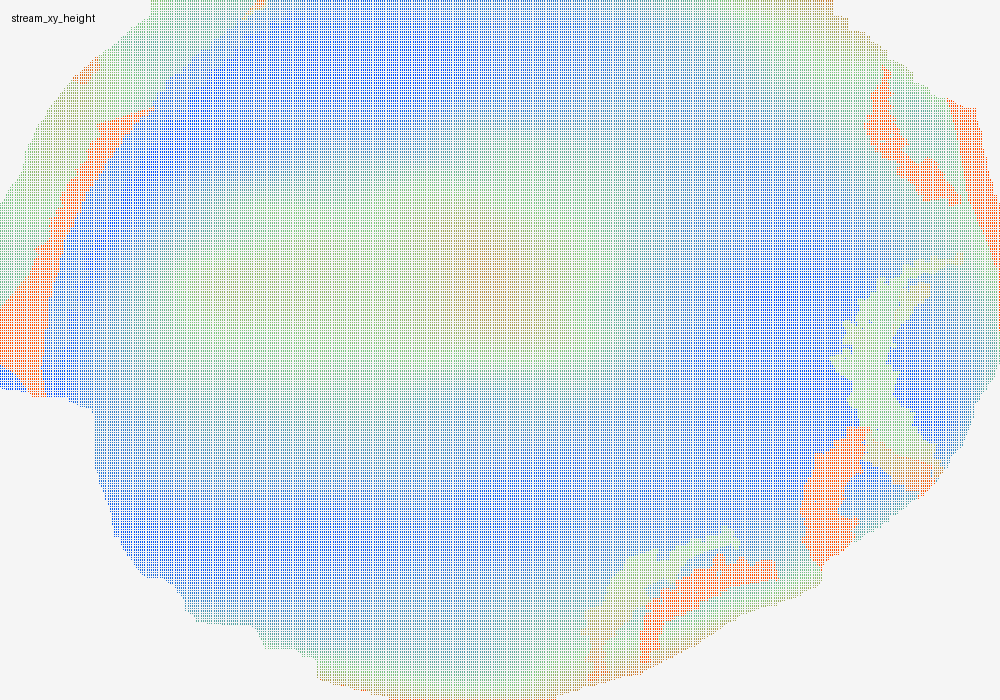
\includegraphics[width=0.47\linewidth]{figures/stream_xy_height.png} &
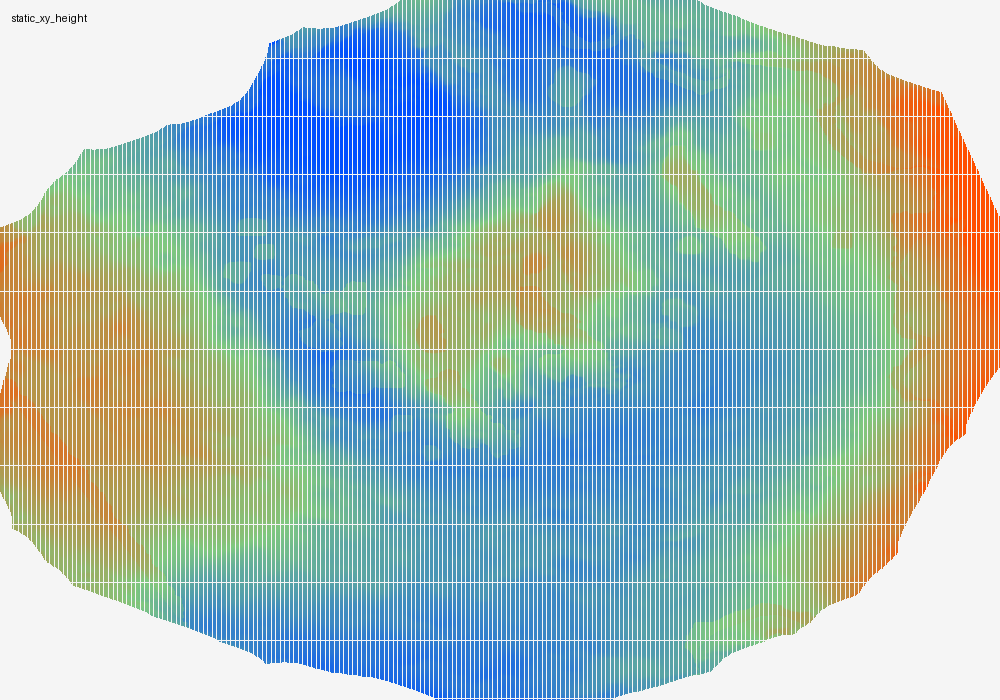
\includegraphics[width=0.47\linewidth]{figures/static_xy_height.png} \\
(a) Streaming preview & (b) Static anchor-canvas reference
\end{tabular}
\caption{XY height projections from the retained comparison. The static reference is denser and uses stronger support filtering; the stream output favors lower latency.}
\label{fig:comparison}
\end{figure*}

\subsection{3-D Reconstruction Metrics to Fill}
Table~\ref{tab:future_3d_metrics} is the planned 3-D reconstruction benchmark table. Values are left as \TBD{} until a metric reference is available. Valid references include a laser scan, structured-light scan, photometric-stereo reconstruction with scale calibration, or a manually validated high-resolution reference.

\begin{table*}[t]
\centering
\caption{Planned 3-D Reconstruction Evaluation. Results are intentionally blank until a metric reference is available.}
\label{tab:future_3d_metrics}
\begin{tabular}{lcccccccc}
\toprule
Method & Points & Acc. $\downarrow$ & Comp. $\downarrow$ & F-score $\uparrow$ & Chamfer $\downarrow$ & Normal Cons. $\uparrow$ & Holes $\downarrow$ & Runtime $\downarrow$ \\
\midrule
Raw OmniVGGT multi-view fusion & \TBD & \TBD & \TBD & \TBD & \TBD & \TBD & \TBD & \TBD \\
Single anchor frame only & \TBD & \TBD & \TBD & \TBD & \TBD & \TBD & \TBD & \TBD \\
Homography canvas, no depth alignment & \TBD & \TBD & \TBD & \TBD & \TBD & \TBD & \TBD & \TBD \\
Anchor canvas with affine depth alignment & \TBD & \TBD & \TBD & \TBD & \TBD & \TBD & \TBD & \TBD \\
Full support-aware anchor canvas & 440,911 & \TBD & \TBD & \TBD & \TBD & \TBD & 0 & \TBD \\
Full method with residual-flow detail & 440,911 & \TBD & \TBD & \TBD & \TBD & \TBD & 0 & \TBD \\
\bottomrule
\end{tabular}
\end{table*}

\subsection{Ablation Plan}
Table~\ref{tab:ablation_plan} lists ablations that should be reported once all variants are regenerated under the same environment. Some variants already exist in old output folders, but a clean paper table should use one consistent script version.

\begin{table*}[t]
\centering
\caption{Planned Ablation Study}
\label{tab:ablation_plan}
\begin{tabular}{lcccccc}
\toprule
Variant & Depth residual MAD $\downarrow$ & Holes $\downarrow$ & Boundary artifacts $\downarrow$ & Duplicate XY $\downarrow$ & Points & Notes \\
\midrule
No depth alignment & \TBD & \TBD & \TBD & \TBD & \TBD & Expected vertical layers \\
Global affine only & \TBD & \TBD & \TBD & \TBD & \TBD & Removes most scale mismatch \\
Local residual correction & \TBD & \TBD & \TBD & \TBD & \TBD & Controls seam residuals \\
No support regularization & \TBD & \TBD & \TBD & \TBD & \TBD & Expected aperture holes \\
No boundary trim & \TBD & \TBD & \TBD & \TBD & \TBD & Expected false edge support \\
Plane residual export & 0.00507 & 0 & \TBD & \TBD & 440,911 & Retained output \\
\bottomrule
\end{tabular}
\end{table*}

\subsection{Reproducibility Checklist}
Each final experiment row should store the following artifacts:
\begin{itemize}
\item input image list and selected keyframe indices;
\item command line and config values;
\item model backend name, precision, target size, and checkpoint path;
\item alignment report with pairwise edges and accepted keyframes;
\item fusion report with per-frame effective weights and support counts;
\item point cloud, projection images, and optional mesh export;
\item scalar metrics as JSON and a markdown report for inspection.
\end{itemize}
This checklist follows the same discipline as the retained local logs. It makes later result replacement mechanical rather than editorial.

\section{Discussion}
\subsection{Why the Added Modules Matter}
The case study supports the central design claim: scene-specific constraints can make a frozen geometry model more usable without changing model weights. The frozen backend supplies depth and confidence. The added modules decide how to align, correct, weight, fuse, and export those predictions. The depth-alignment table is especially direct. Two non-anchor frames become consistent enough for fusion after overlap correction, with median residuals reduced by roughly an order of magnitude.

The anchor-canvas choice also changes the failure surface. Raw 3-D pose fusion can create multiple layers for near-planar sand because each frame may carry a slightly different depth scale. The anchor-canvas representation permits only one height per canonical XY cell. This is not a universal reconstruction model, but it is a strong prior for the inspected surface.

\subsection{Latency Bottleneck}
The stream logs show that model inference dominates. Average fusion time is only 2.37 ms, while the model averages 716 ms in the preview configuration. The system modules therefore add modest overhead relative to the frozen backend. The next latency improvements should come from smaller model windows, compiled backend execution, ONNX/TensorRT export, or lower-resolution preview buckets. The system layer is already structured for these changes because model calls use bucketed shapes.

\subsection{Accuracy and Detail}
The method separates geometry-first output from detail-enhanced output. Plane-residual geometry is defensible because it uses overlap depth correction and a near-planar prior. Residual-flow micro-relief is less certain. It uses multi-view residual motion rather than luminance alone, but its sign and scale are not calibrated. A future metric experiment should report it separately from the geometry-first output.

\subsection{Evaluation Readiness}
The current draft separates implemented diagnostics from future metric claims. Static surface density, hole counts, residual alignment statistics, and streaming latency are available from retained logs. Absolute reconstruction quality, however, requires an external metric reference. This separation is important because it prevents internal visual agreement from being reported as geometric accuracy. Once a reference scan is available, the planned tables can be populated without changing the method definition or baseline taxonomy.

\section{Limitations and Future Work}
The main limitation is lack of metric ground truth. The current evidence is a local case study with logs and internal reference comparisons. It is useful for engineering validation, but it is not enough for a strong reconstruction benchmark claim. A future version should capture the same sand surface with structured light, laser line scanning, calibrated stereo, or photometric stereo with controlled lighting.

The method also assumes a near-planar target. Objects with large relief, self-occlusion, or non-planar topology would require a different representation, such as a full volumetric map or multi-layer surfel model. The current anchor-canvas path intentionally writes only one height per cell.

The final limitation is dependence on feature-based homography alignment. Very low feature count, repeated texture, specular reflection, or severe aperture occlusion can produce bad homographies. The stream path already suppresses unreliable updates, but static reconstruction should add more explicit alignment uncertainty propagation.

Future work should add (i) metric reference capture, (ii) a clean ablation suite regenerated under one code version, (iii) backend acceleration for lower latency, (iv) uncertainty-aware fusion, and (v) support for non-planar inspection surfaces.

\section{Conclusion}
This paper presents an IEEE-style reconstruction study centered on training-free system modules around a frozen geometry foundation model. The method treats OmniVGGT as a local geometry backend and contributes a system layer around it: change-aware streaming, bucketed active windows, protected keyframes, hybrid block mapping, anchor-canvas alignment, overlap-based depth correction, support-aware height-field fusion, and plane-residual export. On the retained sand sequence, the method produces a dense static surface with zero detected internal holes and greatly reduced local depth residuals. The paper also defines a complete 3-D evaluation protocol with placeholder results, so later metric experiments can be inserted without rewriting the methods section.

\section*{Data Availability}
The input sequence, source code, and generated logs are stored in the local project workspace. The reported static values are read from the retained output folder's \texttt{keyframes.json} and \texttt{alignment\_report.json}; the streaming values are read from \texttt{timings.json} and \texttt{comparison.json} under the retained aligned-stream output folder.

\section*{Ethics Statement}
The experiments use non-human scene imagery of a sand surface. No human-subject data or personally identifiable information is involved.

\section*{Author Contributions}
The project author designed the system modules, implemented the reconstruction and streaming pipelines, ran the experiments, and reviewed the manuscript.

\section*{Conflict of Interest}
The author declares no conflict of interest.

\section*{Funding}
No external funding source was recorded in the project materials.

\section*{AI Disclosure}
This manuscript draft was prepared with AI-assisted writing support. Technical claims and numerical results were derived from the project code, local reports, and generated experiment logs, and should be reviewed by the author before submission.

\appendices
\section{Result Fields to Add Before Submission}
Before submission, the placeholders in Tables~\ref{tab:future_3d_metrics} and~\ref{tab:ablation_plan} should be replaced by measurements from a single reproducible evaluation script. The minimum script inputs are a predicted point cloud, a reference point cloud, a scale/alignment transform, a support mask, and a runtime log. The script should save nearest-neighbor distance histograms, precision-recall curves over thresholds, and a JSON file with all scalar metrics.

\section{Suggested Additional Figures}
A final paper should add four visual figures: (i) the input rotating-aperture sequence, (ii) the alignment graph with selected keyframes, (iii) depth residual maps before and after alignment, and (iv) a side-view comparison showing raw multi-layer fusion versus plane-residual output. These figures would make the method easier to inspect than tables alone.

\section{Evaluation Script Skeleton}
The evaluation script should run in five stages. First, load predicted and reference point clouds and remove non-finite points. Second, apply a supplied similarity transform or estimate one from interior support. Third, compute nearest-neighbor distances in both directions with a KD-tree. Fourth, aggregate accuracy, completeness, F-score, Chamfer distance, normal consistency, and surface diagnostics. Fifth, write JSON, markdown, and plots. The output schema should include method name, command, input files, timestamp, point counts, thresholds, and all scalar metrics.

\begin{table}[h]
\centering
\caption{Suggested JSON Metric Fields}
\begin{tabular}{ll}
\toprule
Field & Meaning \\
\midrule
\texttt{points\_pred} & Predicted point count \\
\texttt{points\_ref} & Reference point count \\
\texttt{thresholds} & F-score thresholds \\
\texttt{accuracy} & Mean and thresholded accuracy \\
\texttt{completeness} & Mean and thresholded completeness \\
\texttt{fscore} & F-score per threshold \\
\texttt{chamfer} & Symmetric Chamfer distance \\
\texttt{normal\_consistency} & Normal agreement if available \\
\texttt{hole\_count} & Internal support holes \\
\texttt{seam\_mad} & Boundary seam residual MAD \\
\texttt{runtime} & Timing breakdown \\
\texttt{memory} & CPU and GPU memory report \\
\bottomrule
\end{tabular}
\end{table}

\section{Ablation Command Matrix}
The ablation suite should be generated by changing one factor at a time. A minimal matrix is:
\begin{itemize}
\item \textbf{Depth alignment:} none, global affine, affine plus local residual.
\item \textbf{Fusion:} overwrite, average, confidence-weighted soft fusion.
\item \textbf{Support:} one-frame support, two-frame support, two-frame support with closing.
\item \textbf{Boundary:} no trim, fixed trim, adaptive trim from aperture uncertainty.
\item \textbf{Export:} raw depth, plane residual, plane residual with clipped outliers.
\item \textbf{Detail:} none, residual-flow detail, photometric detail for visualization only.
\end{itemize}
The most useful ablation is not the one with the best-looking picture. It is the one that explains which module removes which failure mode.

\section{Failure-Mode Review Template}
Before final submission, every result figure should be inspected with this checklist:
\begin{itemize}
\item Does the side view show a single thin layer or multiple vertical sheets?
\item Are holes inside the sand support real missing observations or artifacts from deletion?
\item Do aperture edges appear as false physical boundaries?
\item Does residual-flow detail change geometry metrics or only visual texture?
\item Are stream updates skipping frames because the scene is stable or because alignment failed?
\item Are any claims based on the missing \texttt{v5\_support2} directory rather than retained files?
\end{itemize}
This review keeps the paper aligned with the available evidence.

\bibliographystyle{IEEEtran}
\bibliography{references}

\end{document}
